\documentclass[letterpaper,10pt]{article}

\usepackage{enumitem}
\usepackage{titling}
\usepackage{listings}
\usepackage{url}
\usepackage{hyperref}
\usepackage{setspace}
\usepackage{subfig}
\usepackage{sectsty}
\usepackage{pdfpages}
\usepackage{colortbl}
\usepackage{multirow}
\usepackage{multicol}
\usepackage{relsize}
\usepackage{amsmath}
\usepackage{wasysym}
\usepackage{fancyvrb}
\usepackage[yyyymmdd]{datetime}
\usepackage{amsmath,amssymb,amsthm,graphicx,xspace}
\usepackage[titlenotnumbered,noend,noline]{algorithm2e}
\usepackage[compact]{titlesec}
\usepackage{XCharter}
\usepackage[T1]{fontenc}
\usepackage[scaled]{beramono}
\usepackage[normalem]{ulem}
\usepackage{booktabs}
\usepackage{tikz}
\usetikzlibrary{arrows,automata,shapes,trees,matrix,chains,scopes,positioning,calc}
\tikzstyle{block} = [rectangle, draw, fill=blue!20,
text width=2.5em, text centered, rounded corners, minimum height=2em]
\tikzstyle{bw} = [rectangle, draw, fill=blue!20,
text width=4em, text centered, rounded corners, minimum height=2em]

\definecolor{namerow}{cmyk}{.40,.40,.40,.40}
\definecolor{namecol}{cmyk}{.40,.40,.40,.40}
\renewcommand{\dateseparator}{-}

\let\LaTeXtitle\title
\renewcommand{\title}[1]{\LaTeXtitle{\textsf{#1}}}

\lstset{basicstyle=\footnotesize\ttfamily,breaklines=true}

\newcommand{\handout}[5]{
	\noindent
	\begin{center}
		\framebox{
			\vbox{
				\hbox to 5.78in { {\bf ECE 350: Real-Time Operating Systems } \hfill #2 }
				\vspace{4mm}
				\hbox to 5.78in { {\Large \hfill #4  \hfill} }
				\vspace{2mm}
				\hbox to 5.78in { {\em #3 \hfill \today} }
			}
		}
	\end{center}
	\vspace*{4mm}
}

\newcommand{\lecture}[3]{\handout{#1}{#2}{#3}{Lecture#1}}
\newcommand{\tuple}[1]{\ensuremath{\left\langle #1 \right\rangle}\xspace}

\newcommand{\Rplus}{\protect\hspace{-.1em}\protect\raisebox{.35ex}{\smaller{\smaller\textbf{+}}}}
\newcommand{\Cpp}{\mbox{C\Rplus\Rplus}\xspace}


\addtolength{\oddsidemargin}{-1.000in}
\addtolength{\evensidemargin}{-0.500in}
\addtolength{\textwidth}{2.0in}
\addtolength{\topmargin}{-1.000in}
\addtolength{\textheight}{1.75in}
\addtolength{\parskip}{\baselineskip}
\setlength{\parindent}{0in}
\renewcommand{\baselinestretch}{1.5}
\newcommand{\term}{Spring 2023}
\newcommand{\termnumeric}{1235}

\singlespace


\begin{document}

\lecture{ 2 --- Review of Processes and Threads }{\term}{Jeff Zarnett}

\section*{Past is Prologue}
In prerequisite courses (should you have taken them as per the standard program!), we covered three important things that are relevant to the operating system: processes, threads, and hardware. Here, we're going to take some time to review these things and make sure we're on solid ground before moving on. Does this look and sound exactly like what was covered in ECE~252? Yes. But review is necessary.

\subsection*{The Process and the Thread}

A process is a program in execution. It is composed of three things:

\begin{enumerate}
	\item The instructions and data of the program (the compiled executable).
	\item The current state of the program.
	\item Any resources that are needed to execute the program.
\end{enumerate}

Having two instances of the same program running counts as two separate processes. Thus, you may have two windows open for Microsoft Word, and even though they are the same program, they are separate processes. Similarly, two users who both use Firefox at the same time on a terminal server are interacting with two different processes.

\paragraph{The Process Control Block.}
 The operating system's data structure for managing processes is the \textit{Process Control Block} (PCB). This is a data structure containing what the OS needs to know about the program. It is created and updated by the OS for each running process and can be thrown away when the program has finished executing and cleaned everything up. The blocks are held in memory and maintained in some container (e.g., a list) by the kernel.

The process control block will (usually) have~\cite{osi}:
\begin{itemize}
	\item \textbf{Identifier.} A unique ID associated with the process; usually a simple integer that increments when a new process is created and reset when the system is rebooted.
	\item \textbf{State.} The current state of the process.
	\item \textbf{Priority.} How important this process is (compared to the others).
	\item \textbf{Program Counter.} A place to store the address of the next instruction to be executed (*when needed).
	\item \textbf{Register Data.} A place to store the current values of the registers (*when needed); also called context data.
	\item \textbf{Memory Pointers.} Pointers to the code as well as data associated with this process, and any memory that the OS has allocated by request.
	\item \textbf{I/O Status Information.} Any outstanding requests, files, or I/O devices currently assigned to this process.
	\item \textbf{Accounting Information.} Some data about this process's use of resources. This is optional (but common).
\end{itemize}

To represent this visually:

\begin{center}
	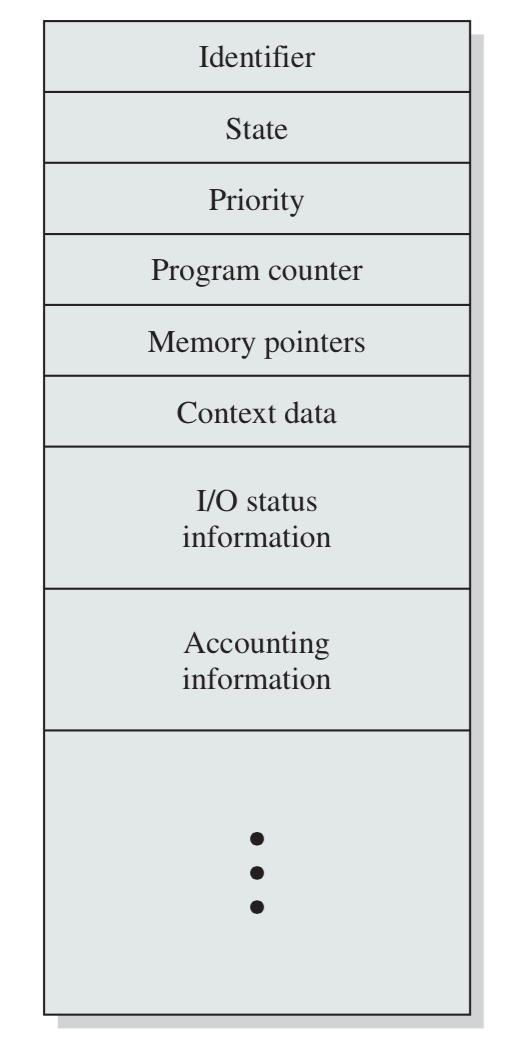
\includegraphics[width=0.24\textwidth]{images/pcb.png}\\
	A simplified Process Control Block~\cite{osi}.
\end{center}

Almost all of the above will be kept up to date constantly as the process executes.  Two of the items, notably the program counter and the register data are asterisked with the words ``when needed''. When the program is running, these values do not need to be updated. However, when a system call (trap) or process switch occurs, and the execution of that process is suspended, the OS will save the state of the process into the PCB. This includes the Program Counter variable (so the program can resume from exactly where it left off) and the Register variables (so the state of the CPU goes back to how it was). The diagram below shows the sequence as the OS switches between the execution of process $P_{0}$ and process $P_{1}$.

\begin{center}
	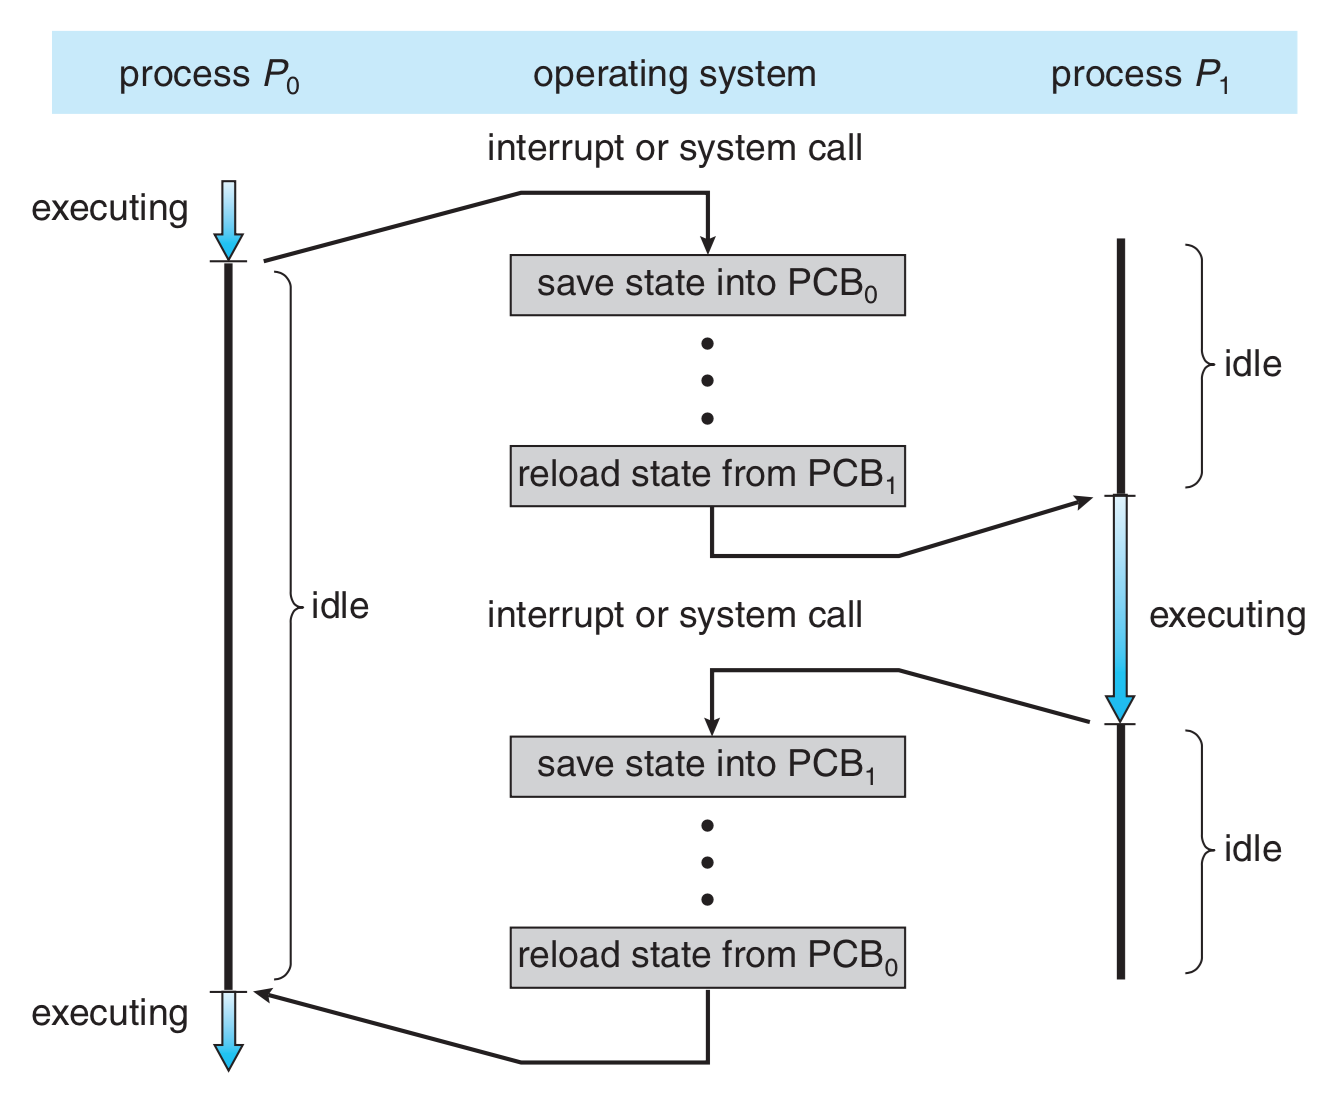
\includegraphics[width=0.65\textwidth]{images/process-switch.png}\\
	A process switch from $P_{0}$ to $P_{1}$ and back again~\cite{osc}.
\end{center}

\paragraph{The Circle of Life.}
Upon creation, the OS will create a new PCB for the process and initialize the data in that block. This means setting the variables to their initial values: setting the initial program state, setting the instruction pointer to the first instruction in \texttt{main}, and so on.  The PCB will then be added to the set of PCBs the OS maintains. After the program is terminated and cleaned up, the OS may collect some data (like a summary of accounting information) and then it can remove the PCB from its list of active processes and carry on.

\subsubsection*{Process Creation}
There are, generally speaking, three main events that may lead to the creation of a process~\cite{mos}:

\begin{enumerate}
	\item System boot up.
	\item User request to start a new process.
	\item One process spawns another.
\end{enumerate}

At boot time the OS starts up various processes, some of which will be in the foreground (visible to the user) and some in the background. A user-visible process might be the log in screen; a background process might be the server that shares media on the local network. The UNIX term for a background process is \textit{Daemon}. You have already worked with one of these if you have ever used the \texttt{ssh} (Secure Shell) command to log into a Linux system; when you attempt to connect it is the \texttt{sshd} (Secure Shell Daemon) that responds to your connection attempt.

Users are well known for starting up processes whenever they feel like it, much to the chagrin of system designers everywhere. Every time you double-click an icon or enter a command line command (like \texttt{ssh} above) that will result in the creation of a process.

An already-executing process may spawn another. If you receive an e-mail with a link in it and click on that link\footnote{Security advice: don't click on links you receive by e-mail.}, the e-mail program will start up the web browser (another process) to open the web page. Or a program may break its work up into different logical parts to be parcelled out to subprograms that run as their own process (to promote parallelism or fault tolerance). When an already-executing program spawns another process, we say the spawning process is the \textit{parent} and the one spawned is the \textit{child}.

Eventually, most processes die. This is sad, but it can happen in one of four ways~\cite{mos}:
\begin{enumerate}
	\item Normal exit (voluntary)
	\item Error exit (voluntary)
	\item Fatal Error (involuntary)
	\item Killed by another process (involuntary)
\end{enumerate}

Most of the time, the process finishes because they are finished or the user asks them to. If the command is to compile some piece of code, when the compiler process is finished, it terminates normally. When you are finished writing a document in a text editor, you may click the close button on the window and this will terminate the program normally.

Sometimes there is voluntary exit, but with an error. If the user attempts to run a program that requires write access to the temporary directory, and it checks for the permission on startup and does not find it, it may exit voluntarily with an error code. Similarly, the compiler will exit with an error if you ask it to compile a non-existent file~\cite{mos}. In either case, the program has chosen to terminate (not continue) because of the error and it is a voluntary termination.

The third reason for termination is a fatal error occurring in the program, like a stack overflow error or division by zero. The OS will detect this error and send it to the program. Very often, this results in the involuntary termination of the offending program. A process may tell the OS it wishes to handle some kinds of errors (like in Java/C\# with the \texttt{try-catch-finally} syntax) in which case the OS will send the error to the program which can hopefully deal with it. If so, the process may continue, otherwise, the unhandled exception will result in the involuntary termination.

The last reason for termination is that one process might be killed by another (yes, processes can murder one another. Is no-one safe?!). Typically this is a user request: a program is stuck or consuming too much CPU and the user opens task manager in Windows or uses the \texttt{ps} command (in UNIX) to find the offender and then terminates it with the ``End Process'' button (in Windows) or the \texttt{kill} command (in UNIX). However, programs can, without user intervention, theoretically kill other processes, such as a parent process killing a child it believes to be stuck (or timed out).

Obviously, there are restrictions on killing process: a user or process must have the rights to execute the victim. Typically a user may only kill a process he or she has created, unless that user is a system administrator. While killing processes may be fun, it is something that should be reserved for when it is needed.

\paragraph{Process States.}

The diagram below shows the five-state model:

\begin{center}
	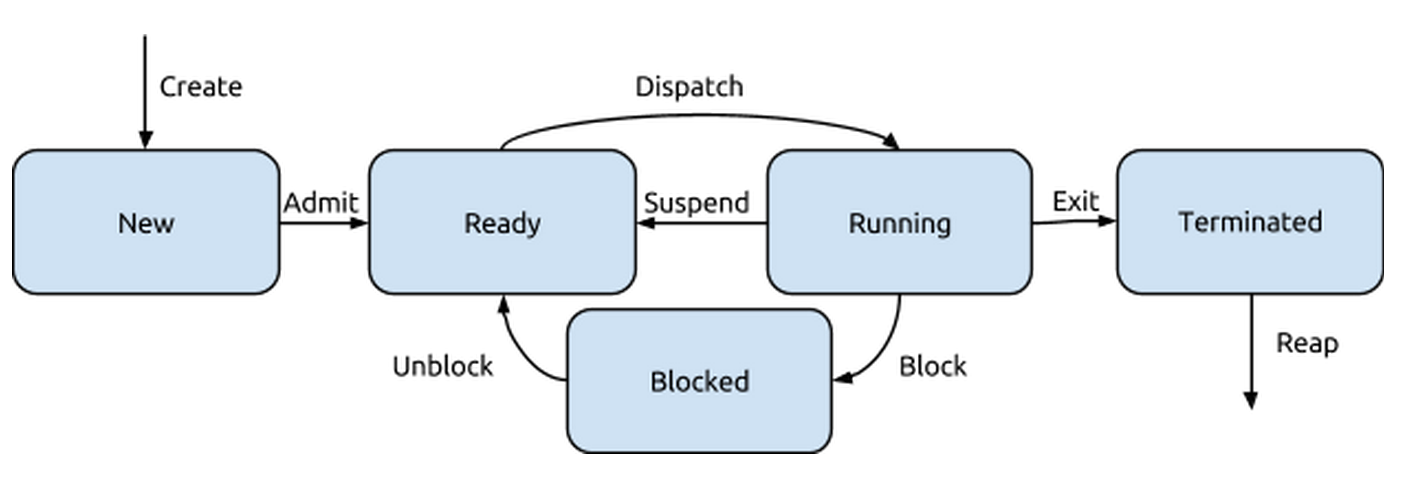
\includegraphics[width=0.85\textwidth]{images/5-state-model.png}\\
	State diagram for the five-state model.
\end{center}

There are now eight transitions, most of which are similar to what we have seen before:

\begin{itemize}
	\item \textbf{Create:} The process is created and enters the New state.
	\item \textbf{Admit:} A process in the New state is added to the list of processes ready to start, in the Ready state.
	\item \textbf{Dispatch:} A process that is not currently running begins executing and moves to the Running state.
	\item \textbf{Suspend:} A running program pauses execution, but can still run if allowed, and moves to the Ready state.
	\item \textbf{Exit:} A running program finishes and moves to the Terminated state; its return value is available.
	\item \textbf{Block:} A running program requests a resource, does not get it right away, and cannot proceed.
	\item \textbf{Unblock:} A program, currently blocked, receives the resource it was waiting for; it moves to the Ready state.
	\item \textbf{Reap:} A terminated program's return value is collected by a \texttt{wait} and its resources can be released.
\end{itemize}

There are two additional ``Exit'' transitions that may happen but are not shown. In theory, a process that is in the Ready or Blocked state might transition directly to the Terminated state. This can happen if a process is killed, by the user or by its parent (recall that parent processes can generally kill their children at any time, something the law thankfully does not permit). It may also happen that the system has a policy of killing all the children of a parent process when the parent process dies.

Remember that this model works for a thread, but the process has two additional ones:

Ready/Swapped (ready to run, and currently not in memory) and Blocked/Swapped (not ready to run, and currently not in memory). That gives us, finally, the seven-state model, a minor variation of the five-state model:

\begin{center}
	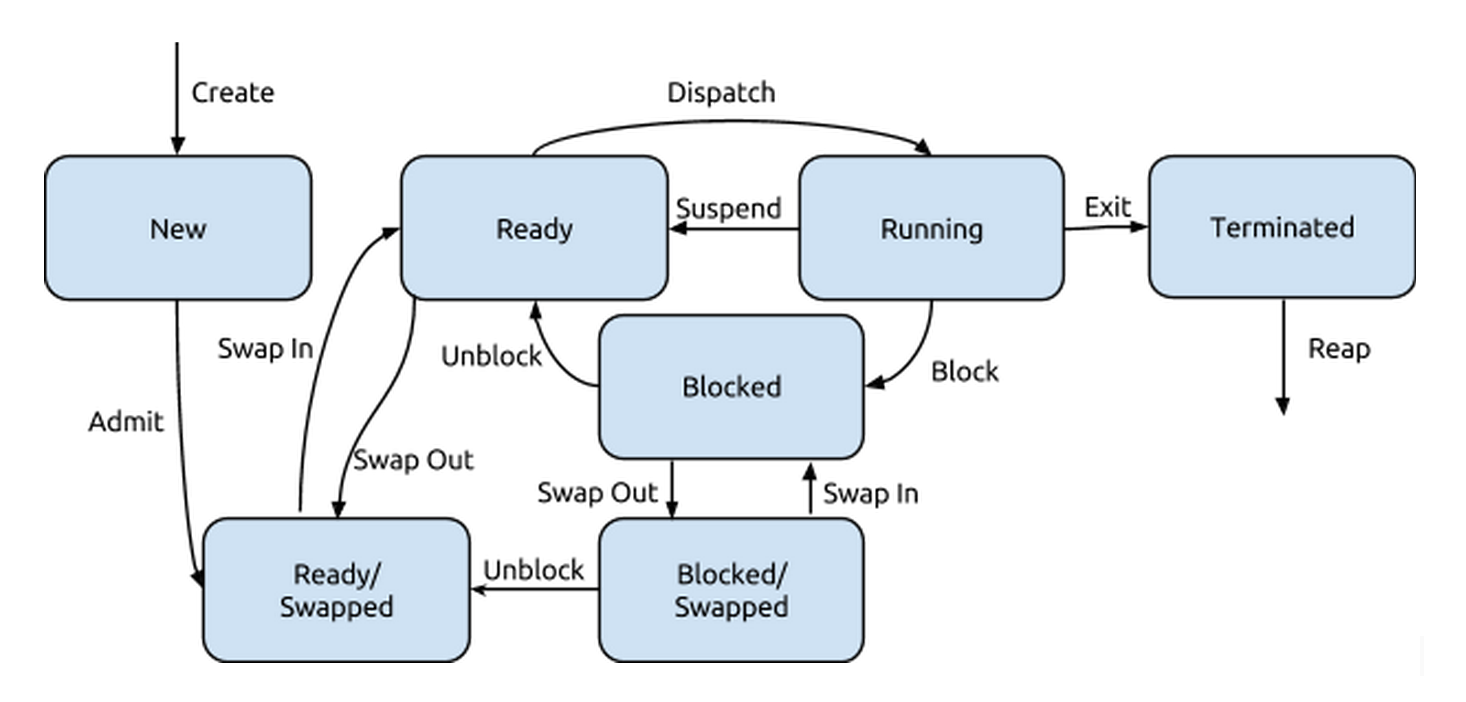
\includegraphics[width=0.85\textwidth]{images/7-state-model.png}\\
	State diagram for the seven-state model.
\end{center}

As in the five-state model, there are additional ``Exit'' transitions that may happen but are not shown. If a process is killed, for example, regardless of whether it is in memory or on disk, it will move to the Terminated state.

At this point I assume you remember how to use \texttt{fork()} and related functions like \texttt{wait()} and there's no need to recap it here. If you are uncertain about it, please check the ECE 252 notes!

\subsection*{And the Thread}

The term ``thread'' is a short form of \textit{Thread of Execution}. A thread of execution is a sequence of executable commands that can be scheduled to run on the CPU. Threads also have some state (where in the sequence of executable commands the program is) and some local variables. Most programs you have written until now probably had only one thread; that is, your program's code is executed one statement at a time, sequentially in some order.

A multithreaded program is one that uses more than one thread, at least some of the time. When a program is started, it begins with an initial thread (where the \texttt{main} function is) and that main thread can create some additional threads if needed. Note that threads can be created and destroyed within a program dynamically: a thread can be created to handle a specific background task, like writing changes to the database, and will terminate when it is done. Or a created thread might be persistent.

In a process that has multiple threads, each thread has its own~\cite{osi}:
\begin{enumerate}
	\item Thread execution state (like process state: running, ready, blocked...).
	\item Saved thread context when not running.
	\item Execution stack.
	\item Local variables.
	\item Access to the memory and resources of the process (shared with all threads in that process).
\end{enumerate}

Or, to represent this visually:

\begin{center}
	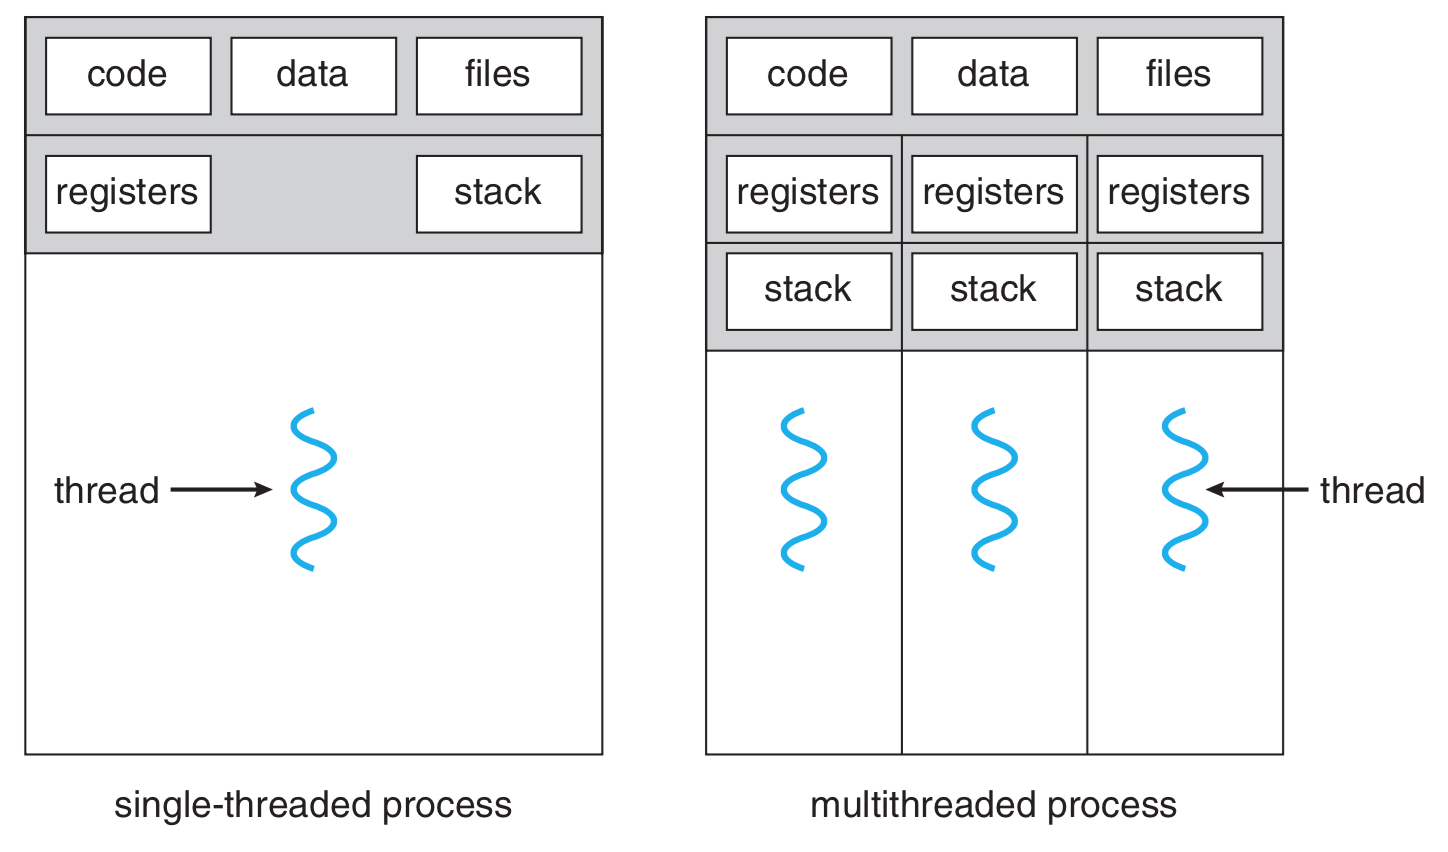
\includegraphics[width=0.625\textwidth]{images/mthread2.png}\\
	A single threaded and a multithreaded process compared side-by-side~\cite{osc}.
\end{center}


As you know, the primary motivation for threads over processes is performance. They are much faster to create and clean up than processes, and there's no overhead of establishing shared-memory communication. But of course, there are risks, like any one thread crashing the whole program. 

Like with processes, I'll assume you remember how the various pthread functions work from ECE 252 -- if not, please go back and look at that -- it will save you a lot of headache...


\bibliographystyle{alphaurl}
\bibliography{350}


\end{document}